\documentclass[9pt]{beamer}
\usepackage[utf8]{inputenc}
\usefonttheme{serif} 
\usefonttheme{structuresmallcapsserif} 
\usepackage{hyperref}
\hypersetup{
    colorlinks=true,
    linkcolor=blue,
    filecolor=magenta,
    urlcolor=cyan,
}

\usetheme{Luebeck}
%\usepackage{media9}
%\usepackage{animate}
\usepackage{multimedia}
\usepackage{textpos} 

\addtobeamertemplate{frametitle}{}{%
    \begin{textblock*}{100mm}(11.75cm,-0.86cm)
        
\includegraphics[height=0.86cm,width=0.86cm]{HIPlogo.png}
    \end{textblock*}
    }
\addtobeamertemplate{frametitle}{}{%
    \begin{textblock*}{100mm}(10.89cm,-0.86cm)
        
\includegraphics[height=0.86cm,width=0.86cm]{HYlogo.jpg}
    \end{textblock*}}
\addtobeamertemplate{frametitle}{}{%
    \begin{textblock*}{100mm}(10.03cm,-0.86cm)
        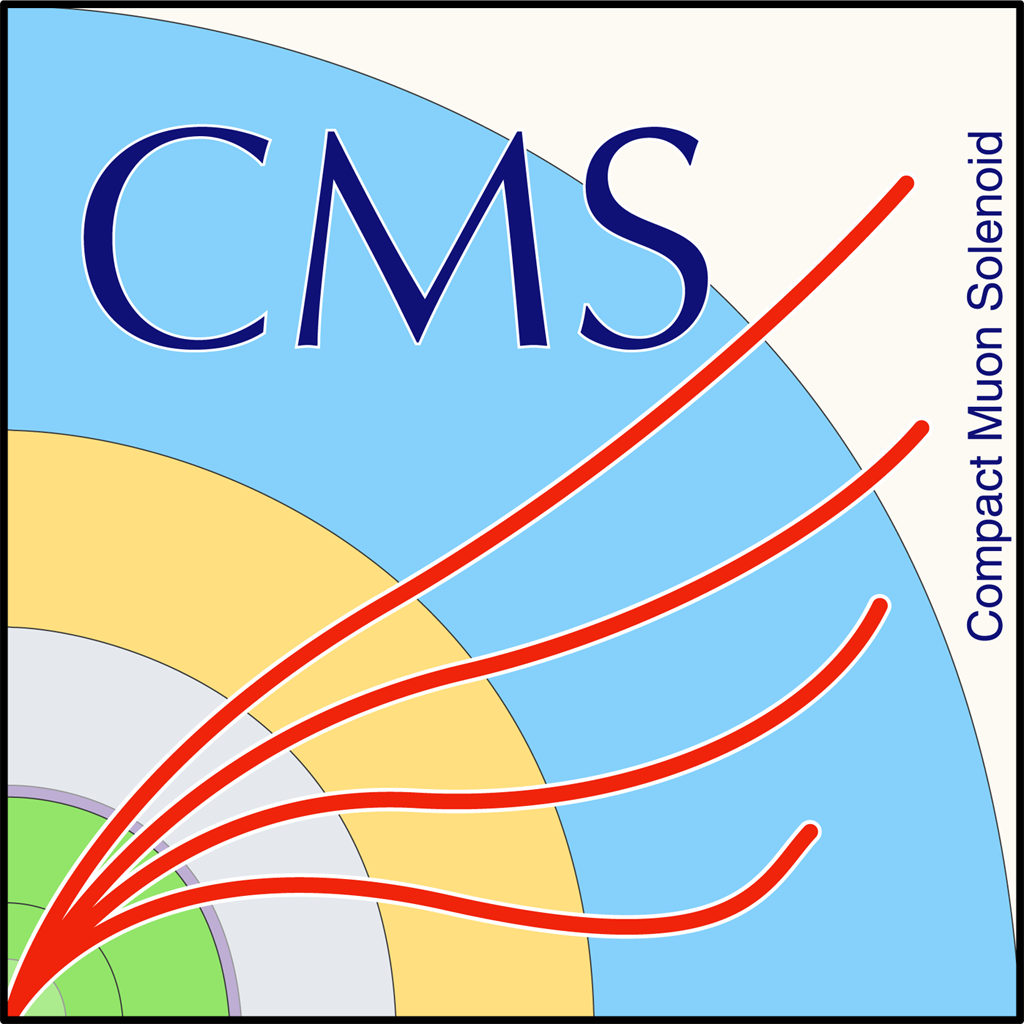
\includegraphics[height=0.86cm,width=0.86cm]{CMSlogo.png}
    \end{textblock*}}

\definecolor{ao}{rgb}{0.0, 0.5, 0.0}
\definecolor{darkgreen}{rgb}{0.0, 0.2, 0.13}
\definecolor{ferngreen}{rgb}{0.31, 0.47, 0.26}
    
\usecolortheme[named=ferngreen]{structure}
\beamertemplatenavigationsymbolsempty
\setbeamertemplate{bibliography item}[text]
\title[BCD16 (Legacy ReReco) hot zones]{BCD16 (Legacy ReReco) hot zones}
%\subtitle{JERC meeting 26th Feb 2018}
\author{Hannu Siikonen}
\institute{Helsinki Institute of Physics \\ \vspace{0.25cm} Instructor Adj.~Prof.~Mikko~Voutilainen}

\date{\today}

\setbeamersize{text margin left=5pt,text margin right=5pt}
\setlength{\labelsep}{12pt}

\begin{document}

\begin{frame}[t]
\titlepage
\end{frame}

\begin{frame}[t]{HLT\_ZeroBias Data}
\begin{columns}[T]
  \begin{column}{.5\textwidth}
  \includegraphics[width=\linewidth]{../pdf/dataquality_relfluctuation_jt0.pdf}
  \end{column}
  \begin{column}{.5\textwidth}
  \includegraphics[width=\linewidth]{../pdf/dataquality_significance_jt0.pdf}
  \end{column}
\end{columns}
\end{frame}

\begin{frame}[t]{HLT\_PFJet40 Data}
\begin{columns}[T]
  \begin{column}{.5\textwidth}
  \includegraphics[width=\linewidth]{../pdf/dataquality_relfluctuation_jt40.pdf}
  \end{column}
  \begin{column}{.5\textwidth}
  \includegraphics[width=\linewidth]{../pdf/dataquality_significance_jt40.pdf}
  \end{column}
\end{columns}
\end{frame}

\begin{frame}[t]{HLT\_PFJet60 Data}
\begin{columns}[T]
  \begin{column}{.5\textwidth}
  \includegraphics[width=\linewidth]{../pdf/dataquality_relfluctuation_jt60.pdf}
  \end{column}
  \begin{column}{.5\textwidth}
  \includegraphics[width=\linewidth]{../pdf/dataquality_significance_jt60.pdf}
  \end{column}
\end{columns}
\end{frame}

\begin{frame}[t]{HLT\_PFJet80 Data}
\begin{columns}[T]
  \begin{column}{.5\textwidth}
  \includegraphics[width=\linewidth]{../pdf/dataquality_relfluctuation_jt80.pdf}
  \end{column}
  \begin{column}{.5\textwidth}
  \includegraphics[width=\linewidth]{../pdf/dataquality_significance_jt80.pdf}
  \end{column}
\end{columns}
\end{frame}

\begin{frame}[t]{HLT\_PFJet140 Data}
\begin{columns}[T]
  \begin{column}{.5\textwidth}
  \includegraphics[width=\linewidth]{../pdf/dataquality_relfluctuation_jt140.pdf}
  \end{column}
  \begin{column}{.5\textwidth}
  \includegraphics[width=\linewidth]{../pdf/dataquality_significance_jt140.pdf}
  \end{column}
\end{columns}
\end{frame}

\begin{frame}[t]{HLT\_PFJet200 Data}
\begin{columns}[T]
  \begin{column}{.5\textwidth}
  \includegraphics[width=\linewidth]{../pdf/dataquality_relfluctuation_jt200.pdf}
  \end{column}
  \begin{column}{.5\textwidth}
  \includegraphics[width=\linewidth]{../pdf/dataquality_significance_jt200.pdf}
  \end{column}
\end{columns}
\end{frame}

\begin{frame}[t]{HLT\_PFJet260 Data}
\begin{columns}[T]
  \begin{column}{.5\textwidth}
  \includegraphics[width=\linewidth]{../pdf/dataquality_relfluctuation_jt260.pdf}
  \end{column}
  \begin{column}{.5\textwidth}
  \includegraphics[width=\linewidth]{../pdf/dataquality_significance_jt260.pdf}
  \end{column}
\end{columns}
\end{frame}

\begin{frame}[t]{HLT\_PFJet320 Data}
\begin{columns}[T]
  \begin{column}{.5\textwidth}
  \includegraphics[width=\linewidth]{../pdf/dataquality_relfluctuation_jt320.pdf}
  \end{column}
  \begin{column}{.5\textwidth}
  \includegraphics[width=\linewidth]{../pdf/dataquality_significance_jt320.pdf}
  \end{column}
\end{columns}
\end{frame}

\begin{frame}[t]{HLT\_PFJet400 Data}
\begin{columns}[T]
  \begin{column}{.5\textwidth}
  \includegraphics[width=\linewidth]{../pdf/dataquality_relfluctuation_jt400.pdf}
  \end{column}
  \begin{column}{.5\textwidth}
  \includegraphics[width=\linewidth]{../pdf/dataquality_significance_jt400.pdf}
  \end{column}
\end{columns}
\end{frame}

\begin{frame}[t]{HLT\_PFJet450 Data}
\begin{columns}[T]
  \begin{column}{.5\textwidth}
  \includegraphics[width=\linewidth]{../pdf/dataquality_relfluctuation_jt450.pdf}
  \end{column}
  \begin{column}{.5\textwidth}
  \includegraphics[width=\linewidth]{../pdf/dataquality_significance_jt450.pdf}
  \end{column}
\end{columns}
\end{frame}

%\begin{frame}[t]{HLT\_PFJet500 Data}
%\begin{columns}[T]
%  \begin{column}{.5\textwidth}
%  \includegraphics[width=\linewidth]{../pdf/dataquality_relfluctuation_jt500.pdf}
%  \end{column}
%  \begin{column}{.5\textwidth}
%  \includegraphics[width=\linewidth]{../pdf/dataquality_significance_jt500.pdf}
%  \end{column}
%\end{columns}
%\end{frame}
%
%\begin{frame}[t]{HLT\_PFJet500 HS1}
%\begin{columns}[T]
%  \begin{column}{.5\textwidth}
%  \includegraphics[width=\linewidth]{../pdf/hwquality_relfluctuation_jt500.pdf}
%  \end{column}
%  \begin{column}{.5\textwidth}
%  \includegraphics[width=\linewidth]{../pdf/hwquality_significance_jt500.pdf}
%  \end{column}
%\end{columns}
%\end{frame}
%
%\begin{frame}[t]{HLT\_PFJet500 P8M1}
%\begin{columns}[T]
%  \begin{column}{.5\textwidth}
%  \includegraphics[width=\linewidth]{../pdf/mcquality_relfluctuation_jt500.pdf}
%  \end{column}
%  \begin{column}{.5\textwidth}
%  \includegraphics[width=\linewidth]{../pdf/mcquality_significance_jt500.pdf}
%  \end{column}
%\end{columns}
%\end{frame}

\begin{frame}[t]{Cumulative summary (HS1,DATA)}
\begin{columns}[T]
  \begin{column}{.5\textwidth}
  \includegraphics[width=\linewidth]{../pdf/hwquality_cumulation.pdf}
  \end{column}
  \begin{column}{.5\textwidth}
  \includegraphics[width=\linewidth]{../pdf/dataquality_cumulation.pdf}
  \end{column}
\end{columns}
\begin{itemize}
 \item Cumulative summary plots over all triggers - attempt to present the excess/deficit plots cumulated over all triggers
 \item In the $\eta$ border zones only the triggers with a sufficient amount of data is used
\end{itemize}
\end{frame}

\begin{frame}[t]{Filtered cumulative summary Data (cold, hot)}
\begin{columns}[T]
  \begin{column}{.5\textwidth}
  \includegraphics[width=\linewidth]{../pdf/dataquality_colds.pdf}
  \end{column}
  \begin{column}{.5\textwidth}
  \includegraphics[width=\linewidth]{../pdf/dataquality_hots.pdf}
  \end{column}
\end{columns}
\begin{itemize}
 \item The same procedure as on the previous slide, but now we emphasize noise that is significant in more than only one trigger
 \item Hot and cold zones separated
\end{itemize}
\end{frame}

\begin{frame}[t]{Filtered cumulative summary HS1 (cold, hot)}
\begin{columns}[T]
  \begin{column}{.5\textwidth}
  \includegraphics[width=\linewidth]{../pdf/hwquality_colds.pdf}
  \end{column}
  \begin{column}{.5\textwidth}
  \includegraphics[width=\linewidth]{../pdf/hwquality_hots.pdf}
  \end{column}
\end{columns}
\begin{itemize}
 \item The same procedure as on the previous slide, but now we emphasize noise that is significant in more than only one trigger
 \item Hot and cold zones separated
\end{itemize}
\end{frame}

\end{document}
